\documentclass[twoside]{book}

% Packages required by doxygen
\usepackage{fixltx2e}
\usepackage{calc}
\usepackage{doxygen}
\usepackage[export]{adjustbox} % also loads graphicx
\usepackage{graphicx}
\usepackage[utf8]{inputenc}
\usepackage{makeidx}
\usepackage{multicol}
\usepackage{multirow}
\PassOptionsToPackage{warn}{textcomp}
\usepackage{textcomp}
\usepackage[nointegrals]{wasysym}
\usepackage[table]{xcolor}

% Font selection
\usepackage[T1]{fontenc}
\usepackage[scaled=.90]{helvet}
\usepackage{courier}
\usepackage{amssymb}
\usepackage{sectsty}
\renewcommand{\familydefault}{\sfdefault}
\allsectionsfont{%
  \fontseries{bc}\selectfont%
  \color{darkgray}%
}
\renewcommand{\DoxyLabelFont}{%
  \fontseries{bc}\selectfont%
  \color{darkgray}%
}
\newcommand{\+}{\discretionary{\mbox{\scriptsize$\hookleftarrow$}}{}{}}

% Page & text layout
\usepackage{geometry}
\geometry{%
  a4paper,%
  top=2.5cm,%
  bottom=2.5cm,%
  left=2.5cm,%
  right=2.5cm%
}
\tolerance=750
\hfuzz=15pt
\hbadness=750
\setlength{\emergencystretch}{15pt}
\setlength{\parindent}{0cm}
\setlength{\parskip}{3ex plus 2ex minus 2ex}
\makeatletter
\renewcommand{\paragraph}{%
  \@startsection{paragraph}{4}{0ex}{-1.0ex}{1.0ex}{%
    \normalfont\normalsize\bfseries\SS@parafont%
  }%
}
\renewcommand{\subparagraph}{%
  \@startsection{subparagraph}{5}{0ex}{-1.0ex}{1.0ex}{%
    \normalfont\normalsize\bfseries\SS@subparafont%
  }%
}
\makeatother

% Headers & footers
\usepackage{fancyhdr}
\pagestyle{fancyplain}
\fancyhead[LE]{\fancyplain{}{\bfseries\thepage}}
\fancyhead[CE]{\fancyplain{}{}}
\fancyhead[RE]{\fancyplain{}{\bfseries\leftmark}}
\fancyhead[LO]{\fancyplain{}{\bfseries\rightmark}}
\fancyhead[CO]{\fancyplain{}{}}
\fancyhead[RO]{\fancyplain{}{\bfseries\thepage}}
\fancyfoot[LE]{\fancyplain{}{}}
\fancyfoot[CE]{\fancyplain{}{}}
\fancyfoot[RE]{\fancyplain{}{\bfseries\scriptsize Generated by Doxygen }}
\fancyfoot[LO]{\fancyplain{}{\bfseries\scriptsize Generated by Doxygen }}
\fancyfoot[CO]{\fancyplain{}{}}
\fancyfoot[RO]{\fancyplain{}{}}
\renewcommand{\footrulewidth}{0.4pt}
\renewcommand{\chaptermark}[1]{%
  \markboth{#1}{}%
}
\renewcommand{\sectionmark}[1]{%
  \markright{\thesection\ #1}%
}

% Indices & bibliography
\usepackage{natbib}
\usepackage[titles]{tocloft}
\setcounter{tocdepth}{3}
\setcounter{secnumdepth}{5}
\makeindex

% Hyperlinks (required, but should be loaded last)
\usepackage{ifpdf}
\ifpdf
  \usepackage[pdftex,pagebackref=true]{hyperref}
\else
  \usepackage[ps2pdf,pagebackref=true]{hyperref}
\fi
\hypersetup{%
  colorlinks=true,%
  linkcolor=blue,%
  citecolor=blue,%
  unicode%
}

% Custom commands
\newcommand{\clearemptydoublepage}{%
  \newpage{\pagestyle{empty}\cleardoublepage}%
}

\usepackage{caption}
\captionsetup{labelsep=space,justification=centering,font={bf},singlelinecheck=off,skip=4pt,position=top}

%===== C O N T E N T S =====

\begin{document}

% Titlepage & ToC
\hypersetup{pageanchor=false,
             bookmarksnumbered=true,
             pdfencoding=unicode
            }
\pagenumbering{alph}
\begin{titlepage}
\vspace*{7cm}
\begin{center}%
{\Large Pozyx\+Positioner }\\
\vspace*{1cm}
{\large Generated by Doxygen 1.8.13}\\
\end{center}
\end{titlepage}
\clearemptydoublepage
\pagenumbering{roman}
\tableofcontents
\clearemptydoublepage
\pagenumbering{arabic}
\hypersetup{pageanchor=true}

%--- Begin generated contents ---
\chapter{Namespace Index}
\section{Packages}
Here are the packages with brief descriptions (if available)\+:\begin{DoxyCompactList}
\item\contentsline{section}{\hyperlink{namespace_pozyx_subscriber}{Pozyx\+Subscriber} }{\pageref{namespace_pozyx_subscriber}}{}
\item\contentsline{section}{\hyperlink{namespace_pozyx_subscriber_1_1_application}{Pozyx\+Subscriber.\+Application} }{\pageref{namespace_pozyx_subscriber_1_1_application}}{}
\item\contentsline{section}{\hyperlink{namespace_pozyx_subscriber_1_1_framework}{Pozyx\+Subscriber.\+Framework} }{\pageref{namespace_pozyx_subscriber_1_1_framework}}{}
\end{DoxyCompactList}

\chapter{Class Index}
\section{Class List}
Here are the classes, structs, unions and interfaces with brief descriptions\+:\begin{DoxyCompactList}
\item\contentsline{section}{\hyperlink{class_pozyx_subscriber_1_1_framework_1_1_anchor}{Pozyx\+Subscriber.\+Framework.\+Anchor} }{\pageref{class_pozyx_subscriber_1_1_framework_1_1_anchor}}{}
\item\contentsline{section}{\hyperlink{class_pozyx_subscriber_1_1_framework_1_1_mqtt_client}{Pozyx\+Subscriber.\+Framework.\+Mqtt\+Client} \\*Mqqt client for subscribing to pozyx broker }{\pageref{class_pozyx_subscriber_1_1_framework_1_1_mqtt_client}}{}
\item\contentsline{section}{\hyperlink{struct_pozyx_subscriber_1_1_framework_1_1_pos_data}{Pozyx\+Subscriber.\+Framework.\+Pos\+Data} \\*Contains a set of position data }{\pageref{struct_pozyx_subscriber_1_1_framework_1_1_pos_data}}{}
\item\contentsline{section}{\hyperlink{struct_pozyx_subscriber_1_1_framework_1_1_pozyx_vector}{Pozyx\+Subscriber.\+Framework.\+Pozyx\+Vector} }{\pageref{struct_pozyx_subscriber_1_1_framework_1_1_pozyx_vector}}{}
\item\contentsline{section}{\hyperlink{class_pozyx_subscriber_1_1_application_1_1_program}{Pozyx\+Subscriber.\+Application.\+Program} }{\pageref{class_pozyx_subscriber_1_1_application_1_1_program}}{}
\item\contentsline{section}{\hyperlink{class_pozyx_subscriber_1_1_framework_1_1_reader}{Pozyx\+Subscriber.\+Framework.\+Reader} \\*Mqqt client for subscribing to pozyx broker }{\pageref{class_pozyx_subscriber_1_1_framework_1_1_reader}}{}
\item\contentsline{section}{\hyperlink{class_pozyx_subscriber_1_1_sim_environment}{Pozyx\+Subscriber.\+Sim\+Environment} \\*Simulation enviornemnt }{\pageref{class_pozyx_subscriber_1_1_sim_environment}}{}
\item\contentsline{section}{\hyperlink{class_pozyx_subscriber_1_1_framework_1_1_sim_object}{Pozyx\+Subscriber.\+Framework.\+Sim\+Object} }{\pageref{class_pozyx_subscriber_1_1_framework_1_1_sim_object}}{}
\item\contentsline{section}{\hyperlink{class_pozyx_subscriber_1_1_framework_1_1_tag}{Pozyx\+Subscriber.\+Framework.\+Tag} }{\pageref{class_pozyx_subscriber_1_1_framework_1_1_tag}}{}
\end{DoxyCompactList}

\chapter{Namespace Documentation}
\hypertarget{namespace_pozyx_positioner}{}\section{Pozyx\+Positioner Namespace Reference}
\label{namespace_pozyx_positioner}\index{Pozyx\+Positioner@{Pozyx\+Positioner}}
\subsection*{Namespaces}
\begin{DoxyCompactItemize}
\item 
namespace \hyperlink{namespace_pozyx_positioner_1_1_application}{Application}
\item 
namespace \hyperlink{namespace_pozyx_positioner_1_1_framework}{Framework}
\end{DoxyCompactItemize}

\hypertarget{namespace_pozyx_positioner_1_1_framework}{}\section{Pozyx\+Positioner.\+Framework Namespace Reference}
\label{namespace_pozyx_positioner_1_1_framework}\index{Pozyx\+Positioner.\+Framework@{Pozyx\+Positioner.\+Framework}}
\subsection*{Classes}
\begin{DoxyCompactItemize}
\item 
class \hyperlink{class_pozyx_positioner_1_1_framework_1_1_mqtt_client}{Mqtt\+Client}
\begin{DoxyCompactList}\small\item\em Mqqt client for subscribing to pozyx broker \end{DoxyCompactList}\item 
struct \hyperlink{struct_pozyx_positioner_1_1_framework_1_1_pos_data}{Pos\+Data}
\begin{DoxyCompactList}\small\item\em Contains a set of position data \end{DoxyCompactList}\item 
struct \hyperlink{struct_pozyx_positioner_1_1_framework_1_1_pozyx_vector}{Pozyx\+Vector}
\item 
class \hyperlink{class_pozyx_positioner_1_1_framework_1_1_sim_environment}{Sim\+Environment}
\begin{DoxyCompactList}\small\item\em Simulation enviornemnt \end{DoxyCompactList}\item 
class \hyperlink{class_pozyx_positioner_1_1_framework_1_1_sim_object}{Sim\+Object}
\item 
class \hyperlink{class_pozyx_positioner_1_1_framework_1_1_tag}{Tag}
\end{DoxyCompactItemize}

\chapter{Class Documentation}
\hypertarget{class_pozyx_positioner_1_1_framework_1_1_mqtt_client}{}\section{Pozyx\+Positioner.\+Framework.\+Mqtt\+Client Class Reference}
\label{class_pozyx_positioner_1_1_framework_1_1_mqtt_client}\index{Pozyx\+Positioner.\+Framework.\+Mqtt\+Client@{Pozyx\+Positioner.\+Framework.\+Mqtt\+Client}}


Mqqt client for subscribing to pozyx broker  




Collaboration diagram for Pozyx\+Positioner.\+Framework.\+Mqtt\+Client\+:
\nopagebreak
\begin{figure}[H]
\begin{center}
\leavevmode
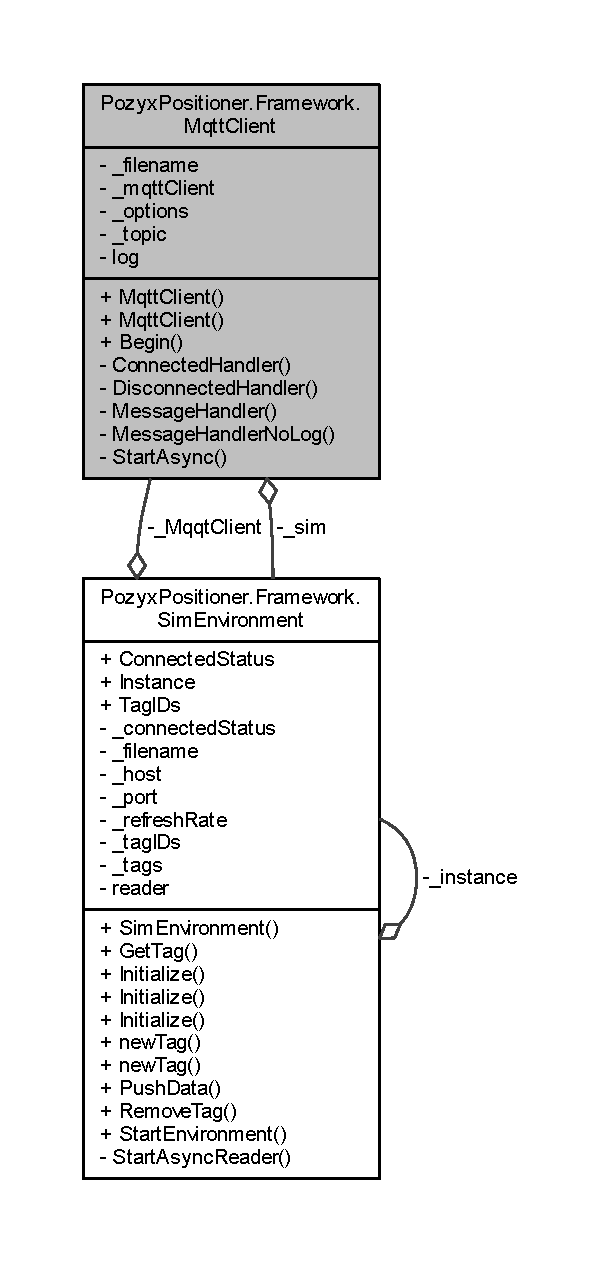
\includegraphics[width=222pt]{class_pozyx_positioner_1_1_framework_1_1_mqtt_client__coll__graph}
\end{center}
\end{figure}
\subsection*{Public Member Functions}
\begin{DoxyCompactItemize}
\item 
\hyperlink{class_pozyx_positioner_1_1_framework_1_1_mqtt_client_a4e2ab3ac03e686e3b85fe50d1a02feb8}{Mqtt\+Client} (string host, int port, \hyperlink{class_pozyx_positioner_1_1_framework_1_1_sim_environment}{Sim\+Environment} Sim)
\begin{DoxyCompactList}\small\item\em Initializes and begins asynch subscription to tag topic from pozyx broker \end{DoxyCompactList}\item 
\hyperlink{class_pozyx_positioner_1_1_framework_1_1_mqtt_client_aed3db79610eeaa328698f435c519c791}{Mqtt\+Client} (string host, int port, \hyperlink{class_pozyx_positioner_1_1_framework_1_1_sim_environment}{Sim\+Environment} Sim, string filename)
\begin{DoxyCompactList}\small\item\em Initializes and begins asynch subscription to tag topic from pozyx broker, one is created by the \hyperlink{class_pozyx_positioner_1_1_framework_1_1_sim_environment}{Sim\+Environment} automatically \end{DoxyCompactList}\item 
void \hyperlink{class_pozyx_positioner_1_1_framework_1_1_mqtt_client_aa08cbaf1de4adeae85b39edc92791ab9}{Begin} ()
\begin{DoxyCompactList}\small\item\em Begins the broker \end{DoxyCompactList}\end{DoxyCompactItemize}


\subsection{Detailed Description}
Mqqt client for subscribing to pozyx broker 



\subsection{Constructor \& Destructor Documentation}
\mbox{\Hypertarget{class_pozyx_positioner_1_1_framework_1_1_mqtt_client_a4e2ab3ac03e686e3b85fe50d1a02feb8}\label{class_pozyx_positioner_1_1_framework_1_1_mqtt_client_a4e2ab3ac03e686e3b85fe50d1a02feb8}} 
\index{Pozyx\+Positioner\+::\+Framework\+::\+Mqtt\+Client@{Pozyx\+Positioner\+::\+Framework\+::\+Mqtt\+Client}!Mqtt\+Client@{Mqtt\+Client}}
\index{Mqtt\+Client@{Mqtt\+Client}!Pozyx\+Positioner\+::\+Framework\+::\+Mqtt\+Client@{Pozyx\+Positioner\+::\+Framework\+::\+Mqtt\+Client}}
\subsubsection{\texorpdfstring{Mqtt\+Client()}{MqttClient()}\hspace{0.1cm}{\footnotesize\ttfamily [1/2]}}
{\footnotesize\ttfamily Pozyx\+Positioner.\+Framework.\+Mqtt\+Client.\+Mqtt\+Client (\begin{DoxyParamCaption}\item[{string}]{host,  }\item[{int}]{port,  }\item[{\hyperlink{class_pozyx_positioner_1_1_framework_1_1_sim_environment}{Sim\+Environment}}]{Sim }\end{DoxyParamCaption})}



Initializes and begins asynch subscription to tag topic from pozyx broker 


\begin{DoxyParams}{Parameters}
{\em host} & Host of the pozyx broker\\
\hline
{\em port} & Port\\
\hline
{\em Sim} & The Simulation object \\
\hline
\end{DoxyParams}
\mbox{\Hypertarget{class_pozyx_positioner_1_1_framework_1_1_mqtt_client_aed3db79610eeaa328698f435c519c791}\label{class_pozyx_positioner_1_1_framework_1_1_mqtt_client_aed3db79610eeaa328698f435c519c791}} 
\index{Pozyx\+Positioner\+::\+Framework\+::\+Mqtt\+Client@{Pozyx\+Positioner\+::\+Framework\+::\+Mqtt\+Client}!Mqtt\+Client@{Mqtt\+Client}}
\index{Mqtt\+Client@{Mqtt\+Client}!Pozyx\+Positioner\+::\+Framework\+::\+Mqtt\+Client@{Pozyx\+Positioner\+::\+Framework\+::\+Mqtt\+Client}}
\subsubsection{\texorpdfstring{Mqtt\+Client()}{MqttClient()}\hspace{0.1cm}{\footnotesize\ttfamily [2/2]}}
{\footnotesize\ttfamily Pozyx\+Positioner.\+Framework.\+Mqtt\+Client.\+Mqtt\+Client (\begin{DoxyParamCaption}\item[{string}]{host,  }\item[{int}]{port,  }\item[{\hyperlink{class_pozyx_positioner_1_1_framework_1_1_sim_environment}{Sim\+Environment}}]{Sim,  }\item[{string}]{filename }\end{DoxyParamCaption})}



Initializes and begins asynch subscription to tag topic from pozyx broker, one is created by the \hyperlink{class_pozyx_positioner_1_1_framework_1_1_sim_environment}{Sim\+Environment} automatically 


\begin{DoxyParams}{Parameters}
{\em host} & Host of the pozyx broker\\
\hline
{\em port} & Port\\
\hline
{\em Sim} & The Simulation object \\
\hline
{\em filename} & The name of a log file \\
\hline
\end{DoxyParams}


\subsection{Member Function Documentation}
\mbox{\Hypertarget{class_pozyx_positioner_1_1_framework_1_1_mqtt_client_aa08cbaf1de4adeae85b39edc92791ab9}\label{class_pozyx_positioner_1_1_framework_1_1_mqtt_client_aa08cbaf1de4adeae85b39edc92791ab9}} 
\index{Pozyx\+Positioner\+::\+Framework\+::\+Mqtt\+Client@{Pozyx\+Positioner\+::\+Framework\+::\+Mqtt\+Client}!Begin@{Begin}}
\index{Begin@{Begin}!Pozyx\+Positioner\+::\+Framework\+::\+Mqtt\+Client@{Pozyx\+Positioner\+::\+Framework\+::\+Mqtt\+Client}}
\subsubsection{\texorpdfstring{Begin()}{Begin()}}
{\footnotesize\ttfamily void Pozyx\+Positioner.\+Framework.\+Mqtt\+Client.\+Begin (\begin{DoxyParamCaption}{ }\end{DoxyParamCaption})}



Begins the broker 

Here is the call graph for this function\+:\nopagebreak
\begin{figure}[H]
\begin{center}
\leavevmode
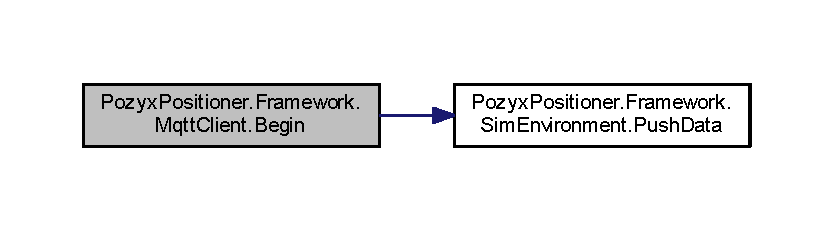
\includegraphics[width=350pt]{class_pozyx_positioner_1_1_framework_1_1_mqtt_client_aa08cbaf1de4adeae85b39edc92791ab9_cgraph}
\end{center}
\end{figure}


The documentation for this class was generated from the following file\+:\begin{DoxyCompactItemize}
\item 
Project/\+Pozyx\+Positioner/\+Pozyx\+Positioner/Subscriber.\+cs\end{DoxyCompactItemize}

\hypertarget{struct_pozyx_positioner_1_1_framework_1_1_pos_data}{}\section{Pozyx\+Positioner.\+Framework.\+Pos\+Data Struct Reference}
\label{struct_pozyx_positioner_1_1_framework_1_1_pos_data}\index{Pozyx\+Positioner.\+Framework.\+Pos\+Data@{Pozyx\+Positioner.\+Framework.\+Pos\+Data}}


Contains a set of position data  




Collaboration diagram for Pozyx\+Positioner.\+Framework.\+Pos\+Data\+:\nopagebreak
\begin{figure}[H]
\begin{center}
\leavevmode
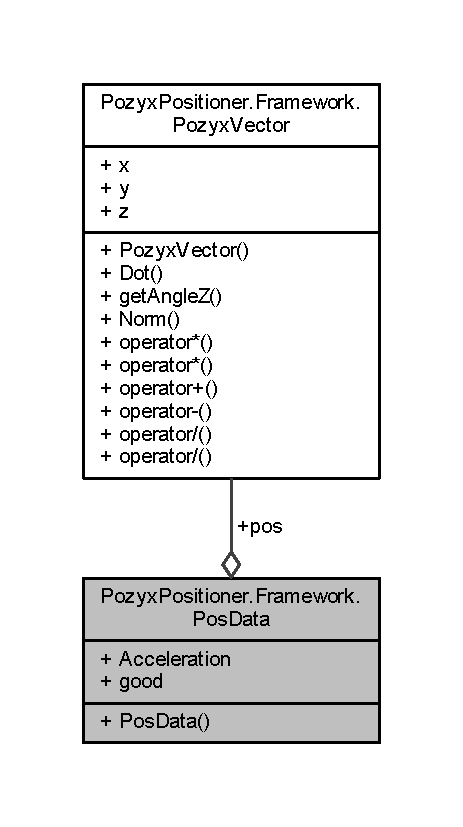
\includegraphics[width=222pt]{struct_pozyx_positioner_1_1_framework_1_1_pos_data__coll__graph}
\end{center}
\end{figure}
\subsection*{Public Member Functions}
\begin{DoxyCompactItemize}
\item 
\hyperlink{struct_pozyx_positioner_1_1_framework_1_1_pos_data_a3a87fee055f3468cb530c7b2cb71098f}{Pos\+Data} (float \+\_\+x, float \+\_\+y, float \+\_\+z)
\begin{DoxyCompactList}\small\item\em Create position data node with x, y, z coordinates \end{DoxyCompactList}\end{DoxyCompactItemize}
\subsection*{Public Attributes}
\begin{DoxyCompactItemize}
\item 
\mbox{\Hypertarget{struct_pozyx_positioner_1_1_framework_1_1_pos_data_a5ad625aaf62369db8ea4cf6943f16686}\label{struct_pozyx_positioner_1_1_framework_1_1_pos_data_a5ad625aaf62369db8ea4cf6943f16686}} 
List$<$ \hyperlink{struct_pozyx_positioner_1_1_framework_1_1_pozyx_vector}{Pozyx\+Vector} $>$ {\bfseries Acceleration}
\item 
\mbox{\Hypertarget{struct_pozyx_positioner_1_1_framework_1_1_pos_data_a4a3b04e06e199ce825d35917fe9a2edb}\label{struct_pozyx_positioner_1_1_framework_1_1_pos_data_a4a3b04e06e199ce825d35917fe9a2edb}} 
bool {\bfseries good}
\item 
\mbox{\Hypertarget{struct_pozyx_positioner_1_1_framework_1_1_pos_data_a2fde856e364bb1dfcc74e654d7eef2f9}\label{struct_pozyx_positioner_1_1_framework_1_1_pos_data_a2fde856e364bb1dfcc74e654d7eef2f9}} 
\hyperlink{struct_pozyx_positioner_1_1_framework_1_1_pozyx_vector}{Pozyx\+Vector} {\bfseries pos}
\end{DoxyCompactItemize}


\subsection{Detailed Description}
Contains a set of position data 



\subsection{Constructor \& Destructor Documentation}
\mbox{\Hypertarget{struct_pozyx_positioner_1_1_framework_1_1_pos_data_a3a87fee055f3468cb530c7b2cb71098f}\label{struct_pozyx_positioner_1_1_framework_1_1_pos_data_a3a87fee055f3468cb530c7b2cb71098f}} 
\index{Pozyx\+Positioner\+::\+Framework\+::\+Pos\+Data@{Pozyx\+Positioner\+::\+Framework\+::\+Pos\+Data}!Pos\+Data@{Pos\+Data}}
\index{Pos\+Data@{Pos\+Data}!Pozyx\+Positioner\+::\+Framework\+::\+Pos\+Data@{Pozyx\+Positioner\+::\+Framework\+::\+Pos\+Data}}
\subsubsection{\texorpdfstring{Pos\+Data()}{PosData()}}
{\footnotesize\ttfamily Pozyx\+Positioner.\+Framework.\+Pos\+Data.\+Pos\+Data (\begin{DoxyParamCaption}\item[{float}]{\+\_\+x,  }\item[{float}]{\+\_\+y,  }\item[{float}]{\+\_\+z }\end{DoxyParamCaption})}



Create position data node with x, y, z coordinates 


\begin{DoxyParams}{Parameters}
{\em \+\_\+x} & \\
\hline
{\em \+\_\+y} & \\
\hline
{\em \+\_\+z} & \\
\hline
\end{DoxyParams}


The documentation for this struct was generated from the following file\+:\begin{DoxyCompactItemize}
\item 
Project/\+Pozyx\+Positioner/\+Pozyx\+Positioner/Pos\+Data.\+cs\end{DoxyCompactItemize}

\hypertarget{struct_pozyx_positioner_1_1_framework_1_1_pozyx_vector}{}\section{Pozyx\+Positioner.\+Framework.\+Pozyx\+Vector Struct Reference}
\label{struct_pozyx_positioner_1_1_framework_1_1_pozyx_vector}\index{Pozyx\+Positioner.\+Framework.\+Pozyx\+Vector@{Pozyx\+Positioner.\+Framework.\+Pozyx\+Vector}}


Collaboration diagram for Pozyx\+Positioner.\+Framework.\+Pozyx\+Vector\+:
\nopagebreak
\begin{figure}[H]
\begin{center}
\leavevmode
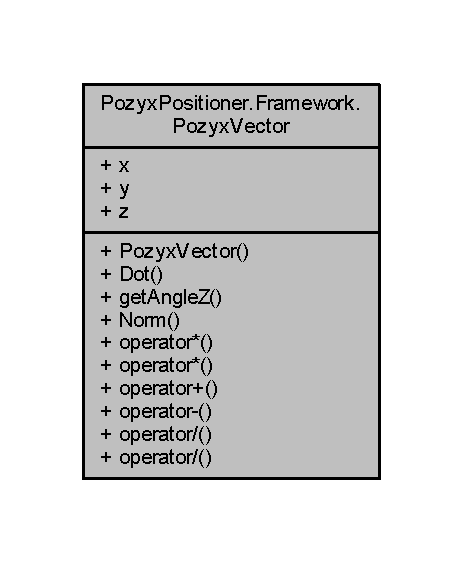
\includegraphics[width=222pt]{struct_pozyx_positioner_1_1_framework_1_1_pozyx_vector__coll__graph}
\end{center}
\end{figure}
\subsection*{Public Member Functions}
\begin{DoxyCompactItemize}
\item 
\mbox{\Hypertarget{struct_pozyx_positioner_1_1_framework_1_1_pozyx_vector_aefc563d4720d301eaf6bd2cb62858c01}\label{struct_pozyx_positioner_1_1_framework_1_1_pozyx_vector_aefc563d4720d301eaf6bd2cb62858c01}} 
{\bfseries Pozyx\+Vector} (float \+\_\+x, float \+\_\+y, float \+\_\+z)
\end{DoxyCompactItemize}
\subsection*{Static Public Member Functions}
\begin{DoxyCompactItemize}
\item 
\mbox{\Hypertarget{struct_pozyx_positioner_1_1_framework_1_1_pozyx_vector_a9f39baf405504f414136b7f9a661dad8}\label{struct_pozyx_positioner_1_1_framework_1_1_pozyx_vector_a9f39baf405504f414136b7f9a661dad8}} 
static float {\bfseries Dot} (\hyperlink{struct_pozyx_positioner_1_1_framework_1_1_pozyx_vector}{Pozyx\+Vector} a, \hyperlink{struct_pozyx_positioner_1_1_framework_1_1_pozyx_vector}{Pozyx\+Vector} b)
\item 
\mbox{\Hypertarget{struct_pozyx_positioner_1_1_framework_1_1_pozyx_vector_a1ba057e7ddbad697e8a8ed6322f8fe7f}\label{struct_pozyx_positioner_1_1_framework_1_1_pozyx_vector_a1ba057e7ddbad697e8a8ed6322f8fe7f}} 
static \hyperlink{struct_pozyx_positioner_1_1_framework_1_1_pozyx_vector}{Pozyx\+Vector} {\bfseries get\+AngleZ} (\hyperlink{struct_pozyx_positioner_1_1_framework_1_1_pozyx_vector}{Pozyx\+Vector} a, \hyperlink{struct_pozyx_positioner_1_1_framework_1_1_pozyx_vector}{Pozyx\+Vector} b)
\item 
\mbox{\Hypertarget{struct_pozyx_positioner_1_1_framework_1_1_pozyx_vector_a1dbaa4407ca3196f8b4de2d86e5ce395}\label{struct_pozyx_positioner_1_1_framework_1_1_pozyx_vector_a1dbaa4407ca3196f8b4de2d86e5ce395}} 
static float {\bfseries Norm} (\hyperlink{struct_pozyx_positioner_1_1_framework_1_1_pozyx_vector}{Pozyx\+Vector} a)
\item 
\mbox{\Hypertarget{struct_pozyx_positioner_1_1_framework_1_1_pozyx_vector_adcd2af121ed12c0d3d0d37c1e06a52c9}\label{struct_pozyx_positioner_1_1_framework_1_1_pozyx_vector_adcd2af121ed12c0d3d0d37c1e06a52c9}} 
static \hyperlink{struct_pozyx_positioner_1_1_framework_1_1_pozyx_vector}{Pozyx\+Vector} {\bfseries operator$\ast$} (\hyperlink{struct_pozyx_positioner_1_1_framework_1_1_pozyx_vector}{Pozyx\+Vector} a, \hyperlink{struct_pozyx_positioner_1_1_framework_1_1_pozyx_vector}{Pozyx\+Vector} b)
\item 
\mbox{\Hypertarget{struct_pozyx_positioner_1_1_framework_1_1_pozyx_vector_a6e4a83f759ad4ded707458ba8da2c4e3}\label{struct_pozyx_positioner_1_1_framework_1_1_pozyx_vector_a6e4a83f759ad4ded707458ba8da2c4e3}} 
static \hyperlink{struct_pozyx_positioner_1_1_framework_1_1_pozyx_vector}{Pozyx\+Vector} {\bfseries operator$\ast$} (\hyperlink{struct_pozyx_positioner_1_1_framework_1_1_pozyx_vector}{Pozyx\+Vector} a, float b)
\item 
\mbox{\Hypertarget{struct_pozyx_positioner_1_1_framework_1_1_pozyx_vector_a73cfc38b2123d1e4dcdd0f9db765c323}\label{struct_pozyx_positioner_1_1_framework_1_1_pozyx_vector_a73cfc38b2123d1e4dcdd0f9db765c323}} 
static \hyperlink{struct_pozyx_positioner_1_1_framework_1_1_pozyx_vector}{Pozyx\+Vector} {\bfseries operator+} (\hyperlink{struct_pozyx_positioner_1_1_framework_1_1_pozyx_vector}{Pozyx\+Vector} a, \hyperlink{struct_pozyx_positioner_1_1_framework_1_1_pozyx_vector}{Pozyx\+Vector} b)
\item 
\mbox{\Hypertarget{struct_pozyx_positioner_1_1_framework_1_1_pozyx_vector_a9f63bedfcb7c16b174e4a7fdae7dc80b}\label{struct_pozyx_positioner_1_1_framework_1_1_pozyx_vector_a9f63bedfcb7c16b174e4a7fdae7dc80b}} 
static \hyperlink{struct_pozyx_positioner_1_1_framework_1_1_pozyx_vector}{Pozyx\+Vector} {\bfseries operator-\/} (\hyperlink{struct_pozyx_positioner_1_1_framework_1_1_pozyx_vector}{Pozyx\+Vector} a, \hyperlink{struct_pozyx_positioner_1_1_framework_1_1_pozyx_vector}{Pozyx\+Vector} b)
\item 
\mbox{\Hypertarget{struct_pozyx_positioner_1_1_framework_1_1_pozyx_vector_aa81e5d2b925c53e58d32833c8bca906e}\label{struct_pozyx_positioner_1_1_framework_1_1_pozyx_vector_aa81e5d2b925c53e58d32833c8bca906e}} 
static \hyperlink{struct_pozyx_positioner_1_1_framework_1_1_pozyx_vector}{Pozyx\+Vector} {\bfseries operator/} (\hyperlink{struct_pozyx_positioner_1_1_framework_1_1_pozyx_vector}{Pozyx\+Vector} a, \hyperlink{struct_pozyx_positioner_1_1_framework_1_1_pozyx_vector}{Pozyx\+Vector} b)
\item 
\mbox{\Hypertarget{struct_pozyx_positioner_1_1_framework_1_1_pozyx_vector_a651734dff7c5e91459beff7ebbea3c6c}\label{struct_pozyx_positioner_1_1_framework_1_1_pozyx_vector_a651734dff7c5e91459beff7ebbea3c6c}} 
static \hyperlink{struct_pozyx_positioner_1_1_framework_1_1_pozyx_vector}{Pozyx\+Vector} {\bfseries operator/} (\hyperlink{struct_pozyx_positioner_1_1_framework_1_1_pozyx_vector}{Pozyx\+Vector} a, float b)
\end{DoxyCompactItemize}
\subsection*{Public Attributes}
\begin{DoxyCompactItemize}
\item 
\mbox{\Hypertarget{struct_pozyx_positioner_1_1_framework_1_1_pozyx_vector_a8d0e8683da20dae755298604eefdae84}\label{struct_pozyx_positioner_1_1_framework_1_1_pozyx_vector_a8d0e8683da20dae755298604eefdae84}} 
float {\bfseries x}
\item 
\mbox{\Hypertarget{struct_pozyx_positioner_1_1_framework_1_1_pozyx_vector_a5e04e95828f39963731121bcb6f62a4c}\label{struct_pozyx_positioner_1_1_framework_1_1_pozyx_vector_a5e04e95828f39963731121bcb6f62a4c}} 
float {\bfseries y}
\item 
\mbox{\Hypertarget{struct_pozyx_positioner_1_1_framework_1_1_pozyx_vector_a1b44279d1786ffde514d431c1521c230}\label{struct_pozyx_positioner_1_1_framework_1_1_pozyx_vector_a1b44279d1786ffde514d431c1521c230}} 
float {\bfseries z}
\end{DoxyCompactItemize}


The documentation for this struct was generated from the following file\+:\begin{DoxyCompactItemize}
\item 
Project/\+Pozyx\+Positioner/\+Pozyx\+Positioner/Vector3\+D\+Node.\+cs\end{DoxyCompactItemize}

\hypertarget{class_pozyx_positioner_1_1_framework_1_1_sim_environment}{}\section{Pozyx\+Positioner.\+Framework.\+Sim\+Environment Class Reference}
\label{class_pozyx_positioner_1_1_framework_1_1_sim_environment}\index{Pozyx\+Positioner.\+Framework.\+Sim\+Environment@{Pozyx\+Positioner.\+Framework.\+Sim\+Environment}}


Simulation enviornemnt  




Collaboration diagram for Pozyx\+Positioner.\+Framework.\+Sim\+Environment\+:
\nopagebreak
\begin{figure}[H]
\begin{center}
\leavevmode
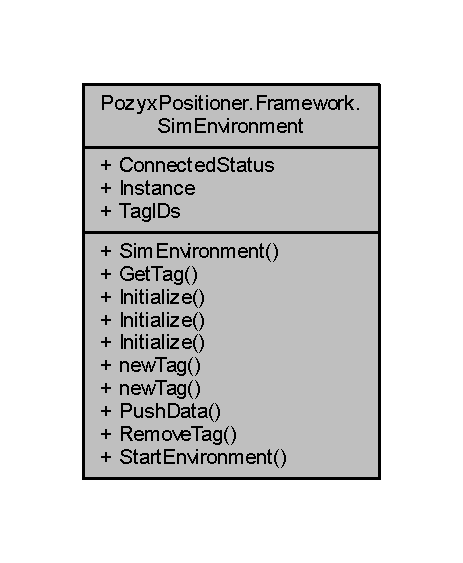
\includegraphics[width=222pt]{class_pozyx_positioner_1_1_framework_1_1_sim_environment__coll__graph}
\end{center}
\end{figure}
\subsection*{Public Member Functions}
\begin{DoxyCompactItemize}
\item 
\hyperlink{class_pozyx_positioner_1_1_framework_1_1_tag}{Tag} \hyperlink{class_pozyx_positioner_1_1_framework_1_1_sim_environment_a2163b3c6c4794224ceba0e5279b7ee8e}{Get\+Tag} (string ID)
\begin{DoxyCompactList}\small\item\em gets a tag from the simulation environment \end{DoxyCompactList}\item 
void \hyperlink{class_pozyx_positioner_1_1_framework_1_1_sim_environment_ad559e17b83e87b9121d3ffd9c08e10b4}{Initialize} (string host, int port, string filename, int refresh\+Rate)
\begin{DoxyCompactList}\small\item\em Simulation Enviorntment Constructor, creates Mqqt\+Client instance, includes a filename to log all messages starting subscription to tags topic \end{DoxyCompactList}\item 
void \hyperlink{class_pozyx_positioner_1_1_framework_1_1_sim_environment_a15a540048be983d1a0ae9983272992be}{Initialize} (string host, int port, int refresh\+Rate)
\begin{DoxyCompactList}\small\item\em Simulation Enviorntment Constructor, creates Mqqt\+Client instance starting subscription to tags topic \end{DoxyCompactList}\item 
void \hyperlink{class_pozyx_positioner_1_1_framework_1_1_sim_environment_a7ede2b3fa6a7af26549b316f1649ba21}{Initialize} (string filename, int refresh\+Rate)
\begin{DoxyCompactList}\small\item\em Simulation Enviorntment Constructor, creates reader instance will send J\+S\+ON strings in coordination to how P\+O\+Z\+YX does using a log file. Simulates reciving tag reads in realtime using a historic log \end{DoxyCompactList}\item 
\hyperlink{class_pozyx_positioner_1_1_framework_1_1_tag}{Tag} \hyperlink{class_pozyx_positioner_1_1_framework_1_1_sim_environment_ad523ae9a258ae7b68d7f966be92ff3bb}{new\+Tag} (string ID, int refresh\+Rate)
\begin{DoxyCompactList}\small\item\em Adds a new tag to the simulation environment \end{DoxyCompactList}\item 
void \hyperlink{class_pozyx_positioner_1_1_framework_1_1_sim_environment_ae804be21b53900cbac13c0cce385b170}{new\+Tag} (\hyperlink{class_pozyx_positioner_1_1_framework_1_1_tag}{Tag} tag)
\begin{DoxyCompactList}\small\item\em Adds a new tag to the simulation environment \end{DoxyCompactList}\item 
void \hyperlink{class_pozyx_positioner_1_1_framework_1_1_sim_environment_a94e341475ddb03c2c27dd253748ad65a}{Push\+Data} (J\+Array msgdata)
\begin{DoxyCompactList}\small\item\em Pushes a J\+S\+ON J\+Array into the simulation \end{DoxyCompactList}\item 
\hyperlink{class_pozyx_positioner_1_1_framework_1_1_tag}{Tag} \hyperlink{class_pozyx_positioner_1_1_framework_1_1_sim_environment_aa69448aa9bc85a646b57b753f5c5e483}{Remove\+Tag} (string ID)
\begin{DoxyCompactList}\small\item\em Removes a tag from the simulation environment \end{DoxyCompactList}\item 
void \hyperlink{class_pozyx_positioner_1_1_framework_1_1_sim_environment_a0d114a29811d19d1376273cb078f6f61}{Start\+Environment} ()
\begin{DoxyCompactList}\small\item\em Start\+Environment method, will begin tracking/reading J\+S\+ON strings and tag readings from Pozyx on a separate thread This begins populating the simulation environment \end{DoxyCompactList}\end{DoxyCompactItemize}
\subsection*{Properties}
\begin{DoxyCompactItemize}
\item 
bool \hyperlink{class_pozyx_positioner_1_1_framework_1_1_sim_environment_ae0d0d204695b423669bd6d0593d961aa}{Connected\+Status}\hspace{0.3cm}{\ttfamily  \mbox{[}get, set\mbox{]}}
\begin{DoxyCompactList}\small\item\em The Connection status of the M\+Q\+TT or Reader class \end{DoxyCompactList}\item 
\mbox{\Hypertarget{class_pozyx_positioner_1_1_framework_1_1_sim_environment_a099b83d9b2af93ae755b7bd081bef37c}\label{class_pozyx_positioner_1_1_framework_1_1_sim_environment_a099b83d9b2af93ae755b7bd081bef37c}} 
static \hyperlink{class_pozyx_positioner_1_1_framework_1_1_sim_environment}{Sim\+Environment} {\bfseries Instance}\hspace{0.3cm}{\ttfamily  \mbox{[}get\mbox{]}}
\item 
List$<$ string $>$ \hyperlink{class_pozyx_positioner_1_1_framework_1_1_sim_environment_af1e5db7ec810b6d92216b74c3eeb657a}{Tag\+I\+Ds}\hspace{0.3cm}{\ttfamily  \mbox{[}get\mbox{]}}
\begin{DoxyCompactList}\small\item\em a list of strings that contain the I\+Ds of all the active tags in the Simulation Environment \end{DoxyCompactList}\end{DoxyCompactItemize}


\subsection{Detailed Description}
Simulation enviornemnt 



\subsection{Member Function Documentation}
\mbox{\Hypertarget{class_pozyx_positioner_1_1_framework_1_1_sim_environment_a2163b3c6c4794224ceba0e5279b7ee8e}\label{class_pozyx_positioner_1_1_framework_1_1_sim_environment_a2163b3c6c4794224ceba0e5279b7ee8e}} 
\index{Pozyx\+Positioner\+::\+Framework\+::\+Sim\+Environment@{Pozyx\+Positioner\+::\+Framework\+::\+Sim\+Environment}!Get\+Tag@{Get\+Tag}}
\index{Get\+Tag@{Get\+Tag}!Pozyx\+Positioner\+::\+Framework\+::\+Sim\+Environment@{Pozyx\+Positioner\+::\+Framework\+::\+Sim\+Environment}}
\subsubsection{\texorpdfstring{Get\+Tag()}{GetTag()}}
{\footnotesize\ttfamily \hyperlink{class_pozyx_positioner_1_1_framework_1_1_tag}{Tag} Pozyx\+Positioner.\+Framework.\+Sim\+Environment.\+Get\+Tag (\begin{DoxyParamCaption}\item[{string}]{ID }\end{DoxyParamCaption})}



gets a tag from the simulation environment 


\begin{DoxyParams}{Parameters}
{\em ID} & the ID of the tag to get\\
\hline
\end{DoxyParams}
\begin{DoxyReturn}{Returns}
the requested tag 
\end{DoxyReturn}
\mbox{\Hypertarget{class_pozyx_positioner_1_1_framework_1_1_sim_environment_ad559e17b83e87b9121d3ffd9c08e10b4}\label{class_pozyx_positioner_1_1_framework_1_1_sim_environment_ad559e17b83e87b9121d3ffd9c08e10b4}} 
\index{Pozyx\+Positioner\+::\+Framework\+::\+Sim\+Environment@{Pozyx\+Positioner\+::\+Framework\+::\+Sim\+Environment}!Initialize@{Initialize}}
\index{Initialize@{Initialize}!Pozyx\+Positioner\+::\+Framework\+::\+Sim\+Environment@{Pozyx\+Positioner\+::\+Framework\+::\+Sim\+Environment}}
\subsubsection{\texorpdfstring{Initialize()}{Initialize()}\hspace{0.1cm}{\footnotesize\ttfamily [1/3]}}
{\footnotesize\ttfamily void Pozyx\+Positioner.\+Framework.\+Sim\+Environment.\+Initialize (\begin{DoxyParamCaption}\item[{string}]{host,  }\item[{int}]{port,  }\item[{string}]{filename,  }\item[{int}]{refresh\+Rate }\end{DoxyParamCaption})}



Simulation Enviorntment Constructor, creates Mqqt\+Client instance, includes a filename to log all messages starting subscription to tags topic 


\begin{DoxyParams}{Parameters}
{\em host} & Local IP addres of Pozyx gateway\\
\hline
{\em port} & Port\\
\hline
{\em filename} & a log file to keep track of all tag messages\\
\hline
{\em refresh\+Rate} & Default refresh rate of a tag not specified by the user\\
\hline
\end{DoxyParams}
\mbox{\Hypertarget{class_pozyx_positioner_1_1_framework_1_1_sim_environment_a15a540048be983d1a0ae9983272992be}\label{class_pozyx_positioner_1_1_framework_1_1_sim_environment_a15a540048be983d1a0ae9983272992be}} 
\index{Pozyx\+Positioner\+::\+Framework\+::\+Sim\+Environment@{Pozyx\+Positioner\+::\+Framework\+::\+Sim\+Environment}!Initialize@{Initialize}}
\index{Initialize@{Initialize}!Pozyx\+Positioner\+::\+Framework\+::\+Sim\+Environment@{Pozyx\+Positioner\+::\+Framework\+::\+Sim\+Environment}}
\subsubsection{\texorpdfstring{Initialize()}{Initialize()}\hspace{0.1cm}{\footnotesize\ttfamily [2/3]}}
{\footnotesize\ttfamily void Pozyx\+Positioner.\+Framework.\+Sim\+Environment.\+Initialize (\begin{DoxyParamCaption}\item[{string}]{host,  }\item[{int}]{port,  }\item[{int}]{refresh\+Rate }\end{DoxyParamCaption})}



Simulation Enviorntment Constructor, creates Mqqt\+Client instance starting subscription to tags topic 


\begin{DoxyParams}{Parameters}
{\em host} & Local IP addres of Pozyx gateway\\
\hline
{\em port} & Port\\
\hline
{\em refresh\+Rate} & Default refresh rate of a tag not specified by the user\\
\hline
\end{DoxyParams}
\mbox{\Hypertarget{class_pozyx_positioner_1_1_framework_1_1_sim_environment_a7ede2b3fa6a7af26549b316f1649ba21}\label{class_pozyx_positioner_1_1_framework_1_1_sim_environment_a7ede2b3fa6a7af26549b316f1649ba21}} 
\index{Pozyx\+Positioner\+::\+Framework\+::\+Sim\+Environment@{Pozyx\+Positioner\+::\+Framework\+::\+Sim\+Environment}!Initialize@{Initialize}}
\index{Initialize@{Initialize}!Pozyx\+Positioner\+::\+Framework\+::\+Sim\+Environment@{Pozyx\+Positioner\+::\+Framework\+::\+Sim\+Environment}}
\subsubsection{\texorpdfstring{Initialize()}{Initialize()}\hspace{0.1cm}{\footnotesize\ttfamily [3/3]}}
{\footnotesize\ttfamily void Pozyx\+Positioner.\+Framework.\+Sim\+Environment.\+Initialize (\begin{DoxyParamCaption}\item[{string}]{filename,  }\item[{int}]{refresh\+Rate }\end{DoxyParamCaption})}



Simulation Enviorntment Constructor, creates reader instance will send J\+S\+ON strings in coordination to how P\+O\+Z\+YX does using a log file. Simulates reciving tag reads in realtime using a historic log 


\begin{DoxyParams}{Parameters}
{\em filename} & name of the log file to simulate with\\
\hline
{\em refresh\+Rate} & Default refresh rate of a tag not specified by the user\\
\hline
\end{DoxyParams}
\mbox{\Hypertarget{class_pozyx_positioner_1_1_framework_1_1_sim_environment_ad523ae9a258ae7b68d7f966be92ff3bb}\label{class_pozyx_positioner_1_1_framework_1_1_sim_environment_ad523ae9a258ae7b68d7f966be92ff3bb}} 
\index{Pozyx\+Positioner\+::\+Framework\+::\+Sim\+Environment@{Pozyx\+Positioner\+::\+Framework\+::\+Sim\+Environment}!new\+Tag@{new\+Tag}}
\index{new\+Tag@{new\+Tag}!Pozyx\+Positioner\+::\+Framework\+::\+Sim\+Environment@{Pozyx\+Positioner\+::\+Framework\+::\+Sim\+Environment}}
\subsubsection{\texorpdfstring{new\+Tag()}{newTag()}\hspace{0.1cm}{\footnotesize\ttfamily [1/2]}}
{\footnotesize\ttfamily \hyperlink{class_pozyx_positioner_1_1_framework_1_1_tag}{Tag} Pozyx\+Positioner.\+Framework.\+Sim\+Environment.\+new\+Tag (\begin{DoxyParamCaption}\item[{string}]{ID,  }\item[{int}]{refresh\+Rate }\end{DoxyParamCaption})}



Adds a new tag to the simulation environment 


\begin{DoxyParams}{Parameters}
{\em ID} & the ID of the tag to add\\
\hline
{\em refresh\+Rate} & the refresh rate of the added tag\\
\hline
\end{DoxyParams}
\begin{DoxyReturn}{Returns}
the newly created tag 
\end{DoxyReturn}
Here is the caller graph for this function\+:\nopagebreak
\begin{figure}[H]
\begin{center}
\leavevmode
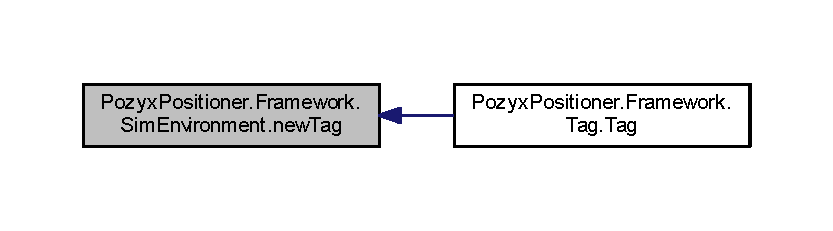
\includegraphics[width=350pt]{class_pozyx_positioner_1_1_framework_1_1_sim_environment_ad523ae9a258ae7b68d7f966be92ff3bb_icgraph}
\end{center}
\end{figure}
\mbox{\Hypertarget{class_pozyx_positioner_1_1_framework_1_1_sim_environment_ae804be21b53900cbac13c0cce385b170}\label{class_pozyx_positioner_1_1_framework_1_1_sim_environment_ae804be21b53900cbac13c0cce385b170}} 
\index{Pozyx\+Positioner\+::\+Framework\+::\+Sim\+Environment@{Pozyx\+Positioner\+::\+Framework\+::\+Sim\+Environment}!new\+Tag@{new\+Tag}}
\index{new\+Tag@{new\+Tag}!Pozyx\+Positioner\+::\+Framework\+::\+Sim\+Environment@{Pozyx\+Positioner\+::\+Framework\+::\+Sim\+Environment}}
\subsubsection{\texorpdfstring{new\+Tag()}{newTag()}\hspace{0.1cm}{\footnotesize\ttfamily [2/2]}}
{\footnotesize\ttfamily void Pozyx\+Positioner.\+Framework.\+Sim\+Environment.\+new\+Tag (\begin{DoxyParamCaption}\item[{\hyperlink{class_pozyx_positioner_1_1_framework_1_1_tag}{Tag}}]{tag }\end{DoxyParamCaption})}



Adds a new tag to the simulation environment 


\begin{DoxyParams}{Parameters}
{\em tag} & the tag to add\\
\hline
\end{DoxyParams}
Here is the call graph for this function\+:\nopagebreak
\begin{figure}[H]
\begin{center}
\leavevmode
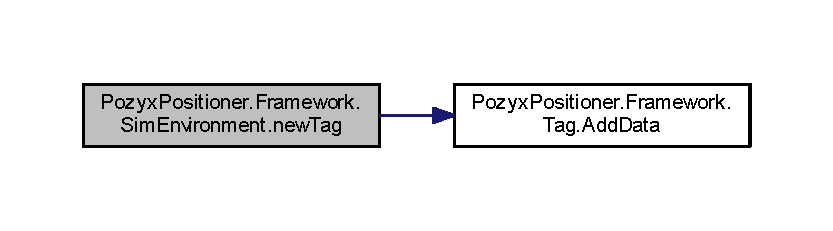
\includegraphics[width=350pt]{class_pozyx_positioner_1_1_framework_1_1_sim_environment_ae804be21b53900cbac13c0cce385b170_cgraph}
\end{center}
\end{figure}
\mbox{\Hypertarget{class_pozyx_positioner_1_1_framework_1_1_sim_environment_a94e341475ddb03c2c27dd253748ad65a}\label{class_pozyx_positioner_1_1_framework_1_1_sim_environment_a94e341475ddb03c2c27dd253748ad65a}} 
\index{Pozyx\+Positioner\+::\+Framework\+::\+Sim\+Environment@{Pozyx\+Positioner\+::\+Framework\+::\+Sim\+Environment}!Push\+Data@{Push\+Data}}
\index{Push\+Data@{Push\+Data}!Pozyx\+Positioner\+::\+Framework\+::\+Sim\+Environment@{Pozyx\+Positioner\+::\+Framework\+::\+Sim\+Environment}}
\subsubsection{\texorpdfstring{Push\+Data()}{PushData()}}
{\footnotesize\ttfamily void Pozyx\+Positioner.\+Framework.\+Sim\+Environment.\+Push\+Data (\begin{DoxyParamCaption}\item[{J\+Array}]{msgdata }\end{DoxyParamCaption})}



Pushes a J\+S\+ON J\+Array into the simulation 


\begin{DoxyParams}{Parameters}
{\em msgdata} & the J\+Array parsed to populate the simulation environment with\\
\hline
\end{DoxyParams}
Here is the caller graph for this function\+:
\nopagebreak
\begin{figure}[H]
\begin{center}
\leavevmode
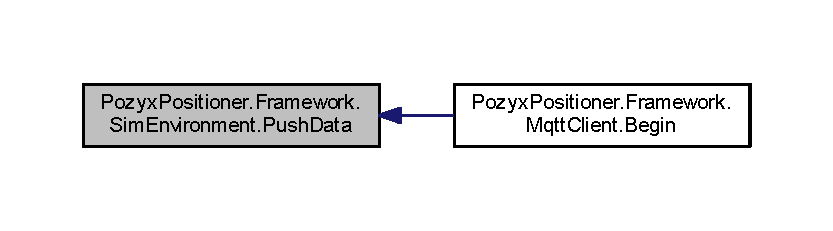
\includegraphics[width=350pt]{class_pozyx_positioner_1_1_framework_1_1_sim_environment_a94e341475ddb03c2c27dd253748ad65a_icgraph}
\end{center}
\end{figure}
\mbox{\Hypertarget{class_pozyx_positioner_1_1_framework_1_1_sim_environment_aa69448aa9bc85a646b57b753f5c5e483}\label{class_pozyx_positioner_1_1_framework_1_1_sim_environment_aa69448aa9bc85a646b57b753f5c5e483}} 
\index{Pozyx\+Positioner\+::\+Framework\+::\+Sim\+Environment@{Pozyx\+Positioner\+::\+Framework\+::\+Sim\+Environment}!Remove\+Tag@{Remove\+Tag}}
\index{Remove\+Tag@{Remove\+Tag}!Pozyx\+Positioner\+::\+Framework\+::\+Sim\+Environment@{Pozyx\+Positioner\+::\+Framework\+::\+Sim\+Environment}}
\subsubsection{\texorpdfstring{Remove\+Tag()}{RemoveTag()}}
{\footnotesize\ttfamily \hyperlink{class_pozyx_positioner_1_1_framework_1_1_tag}{Tag} Pozyx\+Positioner.\+Framework.\+Sim\+Environment.\+Remove\+Tag (\begin{DoxyParamCaption}\item[{string}]{ID }\end{DoxyParamCaption})}



Removes a tag from the simulation environment 


\begin{DoxyParams}{Parameters}
{\em ID} & the ID of the tag to remove\\
\hline
\end{DoxyParams}
\begin{DoxyReturn}{Returns}
the removed tag 
\end{DoxyReturn}
\mbox{\Hypertarget{class_pozyx_positioner_1_1_framework_1_1_sim_environment_a0d114a29811d19d1376273cb078f6f61}\label{class_pozyx_positioner_1_1_framework_1_1_sim_environment_a0d114a29811d19d1376273cb078f6f61}} 
\index{Pozyx\+Positioner\+::\+Framework\+::\+Sim\+Environment@{Pozyx\+Positioner\+::\+Framework\+::\+Sim\+Environment}!Start\+Environment@{Start\+Environment}}
\index{Start\+Environment@{Start\+Environment}!Pozyx\+Positioner\+::\+Framework\+::\+Sim\+Environment@{Pozyx\+Positioner\+::\+Framework\+::\+Sim\+Environment}}
\subsubsection{\texorpdfstring{Start\+Environment()}{StartEnvironment()}}
{\footnotesize\ttfamily void Pozyx\+Positioner.\+Framework.\+Sim\+Environment.\+Start\+Environment (\begin{DoxyParamCaption}{ }\end{DoxyParamCaption})}



Start\+Environment method, will begin tracking/reading J\+S\+ON strings and tag readings from Pozyx on a separate thread This begins populating the simulation environment 



\subsection{Property Documentation}
\mbox{\Hypertarget{class_pozyx_positioner_1_1_framework_1_1_sim_environment_ae0d0d204695b423669bd6d0593d961aa}\label{class_pozyx_positioner_1_1_framework_1_1_sim_environment_ae0d0d204695b423669bd6d0593d961aa}} 
\index{Pozyx\+Positioner\+::\+Framework\+::\+Sim\+Environment@{Pozyx\+Positioner\+::\+Framework\+::\+Sim\+Environment}!Connected\+Status@{Connected\+Status}}
\index{Connected\+Status@{Connected\+Status}!Pozyx\+Positioner\+::\+Framework\+::\+Sim\+Environment@{Pozyx\+Positioner\+::\+Framework\+::\+Sim\+Environment}}
\subsubsection{\texorpdfstring{Connected\+Status}{ConnectedStatus}}
{\footnotesize\ttfamily bool Pozyx\+Positioner.\+Framework.\+Sim\+Environment.\+Connected\+Status\hspace{0.3cm}{\ttfamily [get]}, {\ttfamily [set]}}



The Connection status of the M\+Q\+TT or Reader class 

\mbox{\Hypertarget{class_pozyx_positioner_1_1_framework_1_1_sim_environment_af1e5db7ec810b6d92216b74c3eeb657a}\label{class_pozyx_positioner_1_1_framework_1_1_sim_environment_af1e5db7ec810b6d92216b74c3eeb657a}} 
\index{Pozyx\+Positioner\+::\+Framework\+::\+Sim\+Environment@{Pozyx\+Positioner\+::\+Framework\+::\+Sim\+Environment}!Tag\+I\+Ds@{Tag\+I\+Ds}}
\index{Tag\+I\+Ds@{Tag\+I\+Ds}!Pozyx\+Positioner\+::\+Framework\+::\+Sim\+Environment@{Pozyx\+Positioner\+::\+Framework\+::\+Sim\+Environment}}
\subsubsection{\texorpdfstring{Tag\+I\+Ds}{TagIDs}}
{\footnotesize\ttfamily List$<$string$>$ Pozyx\+Positioner.\+Framework.\+Sim\+Environment.\+Tag\+I\+Ds\hspace{0.3cm}{\ttfamily [get]}}



a list of strings that contain the I\+Ds of all the active tags in the Simulation Environment 



The documentation for this class was generated from the following file\+:\begin{DoxyCompactItemize}
\item 
Project/\+Pozyx\+Positioner/\+Pozyx\+Positioner/Simulation\+Environment.\+cs\end{DoxyCompactItemize}

\hypertarget{class_pozyx_positioner_1_1_framework_1_1_sim_object}{}\section{Pozyx\+Positioner.\+Framework.\+Sim\+Object Class Reference}
\label{class_pozyx_positioner_1_1_framework_1_1_sim_object}\index{Pozyx\+Positioner.\+Framework.\+Sim\+Object@{Pozyx\+Positioner.\+Framework.\+Sim\+Object}}


Collaboration diagram for Pozyx\+Positioner.\+Framework.\+Sim\+Object\+:
\nopagebreak
\begin{figure}[H]
\begin{center}
\leavevmode
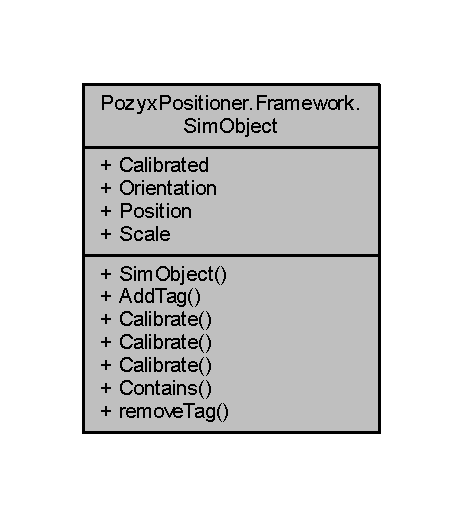
\includegraphics[width=222pt]{class_pozyx_positioner_1_1_framework_1_1_sim_object__coll__graph}
\end{center}
\end{figure}
\subsection*{Public Member Functions}
\begin{DoxyCompactItemize}
\item 
\hyperlink{class_pozyx_positioner_1_1_framework_1_1_sim_object_acc186255ccf8c50a2de3aeaf8e65f645}{Sim\+Object} ()
\begin{DoxyCompactList}\small\item\em \hyperlink{class_pozyx_positioner_1_1_framework_1_1_sim_object}{Sim\+Object} Constructor \end{DoxyCompactList}\item 
void \hyperlink{class_pozyx_positioner_1_1_framework_1_1_sim_object_a46185130a7147410af586622732ad64a}{Add\+Tag} (\hyperlink{class_pozyx_positioner_1_1_framework_1_1_tag}{Tag} tag)
\begin{DoxyCompactList}\small\item\em attaches a tag to this object for tracking, maximum of 2 tags must be attached for orientation measurements \end{DoxyCompactList}\item 
void \hyperlink{class_pozyx_positioner_1_1_framework_1_1_sim_object_ae5a40c80792b6e84ae90cf31e2b5fc8f}{Calibrate} ()
\begin{DoxyCompactList}\small\item\em sets the \hyperlink{class_pozyx_positioner_1_1_framework_1_1_sim_object}{Sim\+Object}\textquotesingle{}s current position and orientation in the real world be the pozyx defaults, and reinitializes its coordinate readings. Sets current real world orientation to 0 Must be done after attaching tags to a \hyperlink{class_pozyx_positioner_1_1_framework_1_1_sim_object}{Sim\+Object}, Simulation\+Environment must be running \end{DoxyCompactList}\item 
void \hyperlink{class_pozyx_positioner_1_1_framework_1_1_sim_object_ad5e3a7c3290c1925d0e7d42a6e8b0111}{Calibrate} (float xpos, float ypos, float zpos)
\begin{DoxyCompactList}\small\item\em sets the \hyperlink{class_pozyx_positioner_1_1_framework_1_1_sim_object}{Sim\+Object}\textquotesingle{}s current position in the real world be the set pos values, and reinitializes its coordinate readings. Sets current real world orientation to 0 Must be done after attaching tags to a \hyperlink{class_pozyx_positioner_1_1_framework_1_1_sim_object}{Sim\+Object}, Simulation\+Environment must be running and connected \end{DoxyCompactList}\item 
void \hyperlink{class_pozyx_positioner_1_1_framework_1_1_sim_object_a7e07ca972f9fc7a962468f9746f9de72}{Calibrate} (float xpos, float ypos, float zpos, float scale)
\begin{DoxyCompactList}\small\item\em sets the \hyperlink{class_pozyx_positioner_1_1_framework_1_1_sim_object}{Sim\+Object}\textquotesingle{}s current position in the real world be the set pos values, and reinitializes its coordinate readings. Sets current real world orientation to 0 Must be done after attaching tags to a \hyperlink{class_pozyx_positioner_1_1_framework_1_1_sim_object}{Sim\+Object}, Simulation\+Environment must be running and connected \end{DoxyCompactList}\item 
bool \hyperlink{class_pozyx_positioner_1_1_framework_1_1_sim_object_a68a000516251ee3062ec72c22cc75f6d}{Contains} (\hyperlink{class_pozyx_positioner_1_1_framework_1_1_tag}{Tag} tag)
\begin{DoxyCompactList}\small\item\em Checks to see if this \hyperlink{class_pozyx_positioner_1_1_framework_1_1_sim_object}{Sim\+Object} has a specific tag attached to it \end{DoxyCompactList}\item 
void \hyperlink{class_pozyx_positioner_1_1_framework_1_1_sim_object_a7cbe138ef2d7a74045a2e706ae3f59b4}{remove\+Tag} (\hyperlink{class_pozyx_positioner_1_1_framework_1_1_tag}{Tag} tag)
\begin{DoxyCompactList}\small\item\em removes a tag from this object \end{DoxyCompactList}\end{DoxyCompactItemize}
\subsection*{Properties}
\begin{DoxyCompactItemize}
\item 
bool \hyperlink{class_pozyx_positioner_1_1_framework_1_1_sim_object_a6bcf32032872002b9edb17f0efc86eef}{Calibrated}\hspace{0.3cm}{\ttfamily  \mbox{[}get\mbox{]}}
\begin{DoxyCompactList}\small\item\em bool\+: is this \hyperlink{class_pozyx_positioner_1_1_framework_1_1_sim_object}{Sim\+Object} is calibrated \end{DoxyCompactList}\item 
\hyperlink{struct_pozyx_positioner_1_1_framework_1_1_pozyx_vector}{Pozyx\+Vector} \hyperlink{class_pozyx_positioner_1_1_framework_1_1_sim_object_af589d7d7066efe823f8a2decd5b081da}{Orientation}\hspace{0.3cm}{\ttfamily  \mbox{[}get\mbox{]}}
\begin{DoxyCompactList}\small\item\em \hyperlink{struct_pozyx_positioner_1_1_framework_1_1_pozyx_vector}{Pozyx\+Vector}\+: The Orientation of the current Simobject in radians in a right handed coordinate system. \end{DoxyCompactList}\item 
\hyperlink{struct_pozyx_positioner_1_1_framework_1_1_pozyx_vector}{Pozyx\+Vector} \hyperlink{class_pozyx_positioner_1_1_framework_1_1_sim_object_a1d2b2ac8c37883939483d4682826db21}{Position}\hspace{0.3cm}{\ttfamily  \mbox{[}get\mbox{]}}
\begin{DoxyCompactList}\small\item\em \hyperlink{struct_pozyx_positioner_1_1_framework_1_1_pozyx_vector}{Pozyx\+Vector}\+: The Position of the current Simobject \end{DoxyCompactList}\item 
float \hyperlink{class_pozyx_positioner_1_1_framework_1_1_sim_object_ab9f89c4e327e25286f0269960d0d2de8}{Scale}\hspace{0.3cm}{\ttfamily  \mbox{[}get, set\mbox{]}}
\begin{DoxyCompactList}\small\item\em float\+: The Scale value of the Object\textquotesingle{}s displacement \end{DoxyCompactList}\end{DoxyCompactItemize}


\subsection{Constructor \& Destructor Documentation}
\mbox{\Hypertarget{class_pozyx_positioner_1_1_framework_1_1_sim_object_acc186255ccf8c50a2de3aeaf8e65f645}\label{class_pozyx_positioner_1_1_framework_1_1_sim_object_acc186255ccf8c50a2de3aeaf8e65f645}} 
\index{Pozyx\+Positioner\+::\+Framework\+::\+Sim\+Object@{Pozyx\+Positioner\+::\+Framework\+::\+Sim\+Object}!Sim\+Object@{Sim\+Object}}
\index{Sim\+Object@{Sim\+Object}!Pozyx\+Positioner\+::\+Framework\+::\+Sim\+Object@{Pozyx\+Positioner\+::\+Framework\+::\+Sim\+Object}}
\subsubsection{\texorpdfstring{Sim\+Object()}{SimObject()}}
{\footnotesize\ttfamily Pozyx\+Positioner.\+Framework.\+Sim\+Object.\+Sim\+Object (\begin{DoxyParamCaption}{ }\end{DoxyParamCaption})}



\hyperlink{class_pozyx_positioner_1_1_framework_1_1_sim_object}{Sim\+Object} Constructor 



\subsection{Member Function Documentation}
\mbox{\Hypertarget{class_pozyx_positioner_1_1_framework_1_1_sim_object_a46185130a7147410af586622732ad64a}\label{class_pozyx_positioner_1_1_framework_1_1_sim_object_a46185130a7147410af586622732ad64a}} 
\index{Pozyx\+Positioner\+::\+Framework\+::\+Sim\+Object@{Pozyx\+Positioner\+::\+Framework\+::\+Sim\+Object}!Add\+Tag@{Add\+Tag}}
\index{Add\+Tag@{Add\+Tag}!Pozyx\+Positioner\+::\+Framework\+::\+Sim\+Object@{Pozyx\+Positioner\+::\+Framework\+::\+Sim\+Object}}
\subsubsection{\texorpdfstring{Add\+Tag()}{AddTag()}}
{\footnotesize\ttfamily void Pozyx\+Positioner.\+Framework.\+Sim\+Object.\+Add\+Tag (\begin{DoxyParamCaption}\item[{\hyperlink{class_pozyx_positioner_1_1_framework_1_1_tag}{Tag}}]{tag }\end{DoxyParamCaption})}



attaches a tag to this object for tracking, maximum of 2 tags must be attached for orientation measurements 


\begin{DoxyParams}{Parameters}
{\em tag} & The tag to attach to the object \\
\hline
\end{DoxyParams}
\mbox{\Hypertarget{class_pozyx_positioner_1_1_framework_1_1_sim_object_ae5a40c80792b6e84ae90cf31e2b5fc8f}\label{class_pozyx_positioner_1_1_framework_1_1_sim_object_ae5a40c80792b6e84ae90cf31e2b5fc8f}} 
\index{Pozyx\+Positioner\+::\+Framework\+::\+Sim\+Object@{Pozyx\+Positioner\+::\+Framework\+::\+Sim\+Object}!Calibrate@{Calibrate}}
\index{Calibrate@{Calibrate}!Pozyx\+Positioner\+::\+Framework\+::\+Sim\+Object@{Pozyx\+Positioner\+::\+Framework\+::\+Sim\+Object}}
\subsubsection{\texorpdfstring{Calibrate()}{Calibrate()}\hspace{0.1cm}{\footnotesize\ttfamily [1/3]}}
{\footnotesize\ttfamily void Pozyx\+Positioner.\+Framework.\+Sim\+Object.\+Calibrate (\begin{DoxyParamCaption}{ }\end{DoxyParamCaption})}



sets the \hyperlink{class_pozyx_positioner_1_1_framework_1_1_sim_object}{Sim\+Object}\textquotesingle{}s current position and orientation in the real world be the pozyx defaults, and reinitializes its coordinate readings. Sets current real world orientation to 0 Must be done after attaching tags to a \hyperlink{class_pozyx_positioner_1_1_framework_1_1_sim_object}{Sim\+Object}, Simulation\+Environment must be running 

\mbox{\Hypertarget{class_pozyx_positioner_1_1_framework_1_1_sim_object_ad5e3a7c3290c1925d0e7d42a6e8b0111}\label{class_pozyx_positioner_1_1_framework_1_1_sim_object_ad5e3a7c3290c1925d0e7d42a6e8b0111}} 
\index{Pozyx\+Positioner\+::\+Framework\+::\+Sim\+Object@{Pozyx\+Positioner\+::\+Framework\+::\+Sim\+Object}!Calibrate@{Calibrate}}
\index{Calibrate@{Calibrate}!Pozyx\+Positioner\+::\+Framework\+::\+Sim\+Object@{Pozyx\+Positioner\+::\+Framework\+::\+Sim\+Object}}
\subsubsection{\texorpdfstring{Calibrate()}{Calibrate()}\hspace{0.1cm}{\footnotesize\ttfamily [2/3]}}
{\footnotesize\ttfamily void Pozyx\+Positioner.\+Framework.\+Sim\+Object.\+Calibrate (\begin{DoxyParamCaption}\item[{float}]{xpos,  }\item[{float}]{ypos,  }\item[{float}]{zpos }\end{DoxyParamCaption})}



sets the \hyperlink{class_pozyx_positioner_1_1_framework_1_1_sim_object}{Sim\+Object}\textquotesingle{}s current position in the real world be the set pos values, and reinitializes its coordinate readings. Sets current real world orientation to 0 Must be done after attaching tags to a \hyperlink{class_pozyx_positioner_1_1_framework_1_1_sim_object}{Sim\+Object}, Simulation\+Environment must be running and connected 


\begin{DoxyParams}{Parameters}
{\em xpos} & the x origin \\
\hline
{\em ypos} & the y origin \\
\hline
{\em zpos} & the z origin \\
\hline
\end{DoxyParams}
\mbox{\Hypertarget{class_pozyx_positioner_1_1_framework_1_1_sim_object_a7e07ca972f9fc7a962468f9746f9de72}\label{class_pozyx_positioner_1_1_framework_1_1_sim_object_a7e07ca972f9fc7a962468f9746f9de72}} 
\index{Pozyx\+Positioner\+::\+Framework\+::\+Sim\+Object@{Pozyx\+Positioner\+::\+Framework\+::\+Sim\+Object}!Calibrate@{Calibrate}}
\index{Calibrate@{Calibrate}!Pozyx\+Positioner\+::\+Framework\+::\+Sim\+Object@{Pozyx\+Positioner\+::\+Framework\+::\+Sim\+Object}}
\subsubsection{\texorpdfstring{Calibrate()}{Calibrate()}\hspace{0.1cm}{\footnotesize\ttfamily [3/3]}}
{\footnotesize\ttfamily void Pozyx\+Positioner.\+Framework.\+Sim\+Object.\+Calibrate (\begin{DoxyParamCaption}\item[{float}]{xpos,  }\item[{float}]{ypos,  }\item[{float}]{zpos,  }\item[{float}]{scale }\end{DoxyParamCaption})}



sets the \hyperlink{class_pozyx_positioner_1_1_framework_1_1_sim_object}{Sim\+Object}\textquotesingle{}s current position in the real world be the set pos values, and reinitializes its coordinate readings. Sets current real world orientation to 0 Must be done after attaching tags to a \hyperlink{class_pozyx_positioner_1_1_framework_1_1_sim_object}{Sim\+Object}, Simulation\+Environment must be running and connected 


\begin{DoxyParams}{Parameters}
{\em xpos} & the x origin \\
\hline
{\em ypos} & the y origin \\
\hline
{\em zpos} & the z origin \\
\hline
{\em scale} & the scale of the position\textquotesingle{}s displacement \\
\hline
\end{DoxyParams}
\mbox{\Hypertarget{class_pozyx_positioner_1_1_framework_1_1_sim_object_a68a000516251ee3062ec72c22cc75f6d}\label{class_pozyx_positioner_1_1_framework_1_1_sim_object_a68a000516251ee3062ec72c22cc75f6d}} 
\index{Pozyx\+Positioner\+::\+Framework\+::\+Sim\+Object@{Pozyx\+Positioner\+::\+Framework\+::\+Sim\+Object}!Contains@{Contains}}
\index{Contains@{Contains}!Pozyx\+Positioner\+::\+Framework\+::\+Sim\+Object@{Pozyx\+Positioner\+::\+Framework\+::\+Sim\+Object}}
\subsubsection{\texorpdfstring{Contains()}{Contains()}}
{\footnotesize\ttfamily bool Pozyx\+Positioner.\+Framework.\+Sim\+Object.\+Contains (\begin{DoxyParamCaption}\item[{\hyperlink{class_pozyx_positioner_1_1_framework_1_1_tag}{Tag}}]{tag }\end{DoxyParamCaption})}



Checks to see if this \hyperlink{class_pozyx_positioner_1_1_framework_1_1_sim_object}{Sim\+Object} has a specific tag attached to it 


\begin{DoxyParams}{Parameters}
{\em tag} & The tag to check \\
\hline
\end{DoxyParams}
\begin{DoxyReturn}{Returns}
True if tag is attached 
\end{DoxyReturn}
\mbox{\Hypertarget{class_pozyx_positioner_1_1_framework_1_1_sim_object_a7cbe138ef2d7a74045a2e706ae3f59b4}\label{class_pozyx_positioner_1_1_framework_1_1_sim_object_a7cbe138ef2d7a74045a2e706ae3f59b4}} 
\index{Pozyx\+Positioner\+::\+Framework\+::\+Sim\+Object@{Pozyx\+Positioner\+::\+Framework\+::\+Sim\+Object}!remove\+Tag@{remove\+Tag}}
\index{remove\+Tag@{remove\+Tag}!Pozyx\+Positioner\+::\+Framework\+::\+Sim\+Object@{Pozyx\+Positioner\+::\+Framework\+::\+Sim\+Object}}
\subsubsection{\texorpdfstring{remove\+Tag()}{removeTag()}}
{\footnotesize\ttfamily void Pozyx\+Positioner.\+Framework.\+Sim\+Object.\+remove\+Tag (\begin{DoxyParamCaption}\item[{\hyperlink{class_pozyx_positioner_1_1_framework_1_1_tag}{Tag}}]{tag }\end{DoxyParamCaption})}



removes a tag from this object 


\begin{DoxyParams}{Parameters}
{\em tag} & The tag to remove \\
\hline
\end{DoxyParams}


\subsection{Property Documentation}
\mbox{\Hypertarget{class_pozyx_positioner_1_1_framework_1_1_sim_object_a6bcf32032872002b9edb17f0efc86eef}\label{class_pozyx_positioner_1_1_framework_1_1_sim_object_a6bcf32032872002b9edb17f0efc86eef}} 
\index{Pozyx\+Positioner\+::\+Framework\+::\+Sim\+Object@{Pozyx\+Positioner\+::\+Framework\+::\+Sim\+Object}!Calibrated@{Calibrated}}
\index{Calibrated@{Calibrated}!Pozyx\+Positioner\+::\+Framework\+::\+Sim\+Object@{Pozyx\+Positioner\+::\+Framework\+::\+Sim\+Object}}
\subsubsection{\texorpdfstring{Calibrated}{Calibrated}}
{\footnotesize\ttfamily bool Pozyx\+Positioner.\+Framework.\+Sim\+Object.\+Calibrated\hspace{0.3cm}{\ttfamily [get]}}



bool\+: is this \hyperlink{class_pozyx_positioner_1_1_framework_1_1_sim_object}{Sim\+Object} is calibrated 

\mbox{\Hypertarget{class_pozyx_positioner_1_1_framework_1_1_sim_object_af589d7d7066efe823f8a2decd5b081da}\label{class_pozyx_positioner_1_1_framework_1_1_sim_object_af589d7d7066efe823f8a2decd5b081da}} 
\index{Pozyx\+Positioner\+::\+Framework\+::\+Sim\+Object@{Pozyx\+Positioner\+::\+Framework\+::\+Sim\+Object}!Orientation@{Orientation}}
\index{Orientation@{Orientation}!Pozyx\+Positioner\+::\+Framework\+::\+Sim\+Object@{Pozyx\+Positioner\+::\+Framework\+::\+Sim\+Object}}
\subsubsection{\texorpdfstring{Orientation}{Orientation}}
{\footnotesize\ttfamily \hyperlink{struct_pozyx_positioner_1_1_framework_1_1_pozyx_vector}{Pozyx\+Vector} Pozyx\+Positioner.\+Framework.\+Sim\+Object.\+Orientation\hspace{0.3cm}{\ttfamily [get]}}



\hyperlink{struct_pozyx_positioner_1_1_framework_1_1_pozyx_vector}{Pozyx\+Vector}\+: The Orientation of the current Simobject in radians in a right handed coordinate system. 

\mbox{\Hypertarget{class_pozyx_positioner_1_1_framework_1_1_sim_object_a1d2b2ac8c37883939483d4682826db21}\label{class_pozyx_positioner_1_1_framework_1_1_sim_object_a1d2b2ac8c37883939483d4682826db21}} 
\index{Pozyx\+Positioner\+::\+Framework\+::\+Sim\+Object@{Pozyx\+Positioner\+::\+Framework\+::\+Sim\+Object}!Position@{Position}}
\index{Position@{Position}!Pozyx\+Positioner\+::\+Framework\+::\+Sim\+Object@{Pozyx\+Positioner\+::\+Framework\+::\+Sim\+Object}}
\subsubsection{\texorpdfstring{Position}{Position}}
{\footnotesize\ttfamily \hyperlink{struct_pozyx_positioner_1_1_framework_1_1_pozyx_vector}{Pozyx\+Vector} Pozyx\+Positioner.\+Framework.\+Sim\+Object.\+Position\hspace{0.3cm}{\ttfamily [get]}}



\hyperlink{struct_pozyx_positioner_1_1_framework_1_1_pozyx_vector}{Pozyx\+Vector}\+: The Position of the current Simobject 

\mbox{\Hypertarget{class_pozyx_positioner_1_1_framework_1_1_sim_object_ab9f89c4e327e25286f0269960d0d2de8}\label{class_pozyx_positioner_1_1_framework_1_1_sim_object_ab9f89c4e327e25286f0269960d0d2de8}} 
\index{Pozyx\+Positioner\+::\+Framework\+::\+Sim\+Object@{Pozyx\+Positioner\+::\+Framework\+::\+Sim\+Object}!Scale@{Scale}}
\index{Scale@{Scale}!Pozyx\+Positioner\+::\+Framework\+::\+Sim\+Object@{Pozyx\+Positioner\+::\+Framework\+::\+Sim\+Object}}
\subsubsection{\texorpdfstring{Scale}{Scale}}
{\footnotesize\ttfamily float Pozyx\+Positioner.\+Framework.\+Sim\+Object.\+Scale\hspace{0.3cm}{\ttfamily [get]}, {\ttfamily [set]}}



float\+: The Scale value of the Object\textquotesingle{}s displacement 



The documentation for this class was generated from the following file\+:\begin{DoxyCompactItemize}
\item 
Project/\+Pozyx\+Positioner/\+Pozyx\+Positioner/Sim\+Object.\+cs\end{DoxyCompactItemize}

\hypertarget{class_pozyx_positioner_1_1_framework_1_1_tag}{}\section{Pozyx\+Positioner.\+Framework.\+Tag Class Reference}
\label{class_pozyx_positioner_1_1_framework_1_1_tag}\index{Pozyx\+Positioner.\+Framework.\+Tag@{Pozyx\+Positioner.\+Framework.\+Tag}}


Collaboration diagram for Pozyx\+Positioner.\+Framework.\+Tag\+:
\nopagebreak
\begin{figure}[H]
\begin{center}
\leavevmode
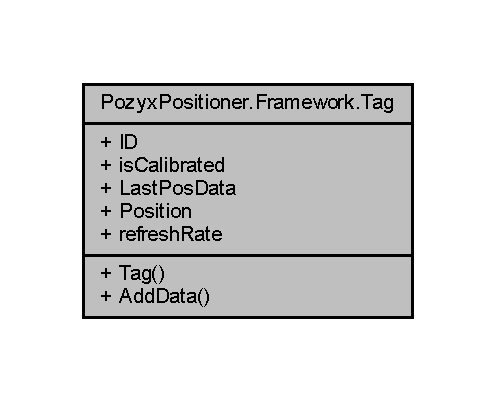
\includegraphics[width=238pt]{class_pozyx_positioner_1_1_framework_1_1_tag__coll__graph}
\end{center}
\end{figure}
\subsection*{Public Member Functions}
\begin{DoxyCompactItemize}
\item 
\hyperlink{class_pozyx_positioner_1_1_framework_1_1_tag_a9b58a1a5756bf3c8cda1e2afd32276b2}{Tag} (string \hyperlink{class_pozyx_positioner_1_1_framework_1_1_tag_a0d75eeca4dea7088e2b4a60230c13012}{ID}, int Refresh\+Rate)
\begin{DoxyCompactList}\small\item\em \hyperlink{class_pozyx_positioner_1_1_framework_1_1_tag}{Tag} Constructor \end{DoxyCompactList}\item 
void \hyperlink{class_pozyx_positioner_1_1_framework_1_1_tag_ac2741e137c420ad71f64ee2d3d5fefe8}{Add\+Data} (\hyperlink{struct_pozyx_positioner_1_1_framework_1_1_pos_data}{Pos\+Data} data)
\begin{DoxyCompactList}\small\item\em Adds data to this tag\textquotesingle{}s positional data list, normalizes the data. Then calculates the best possible realtime position \end{DoxyCompactList}\end{DoxyCompactItemize}
\subsection*{Properties}
\begin{DoxyCompactItemize}
\item 
string \hyperlink{class_pozyx_positioner_1_1_framework_1_1_tag_a0d75eeca4dea7088e2b4a60230c13012}{ID}\hspace{0.3cm}{\ttfamily  \mbox{[}get\mbox{]}}
\begin{DoxyCompactList}\small\item\em the ID of the tag \end{DoxyCompactList}\item 
\mbox{\Hypertarget{class_pozyx_positioner_1_1_framework_1_1_tag_a02cdde9c3303a18f28453056939bf045}\label{class_pozyx_positioner_1_1_framework_1_1_tag_a02cdde9c3303a18f28453056939bf045}} 
bool {\bfseries is\+Calibrated}\hspace{0.3cm}{\ttfamily  \mbox{[}get, set\mbox{]}}
\item 
\hyperlink{struct_pozyx_positioner_1_1_framework_1_1_pozyx_vector}{Pozyx\+Vector} \hyperlink{class_pozyx_positioner_1_1_framework_1_1_tag_a0b1b836b4e64ae70171587a2bcde4d71}{Position}\hspace{0.3cm}{\ttfamily  \mbox{[}get\mbox{]}}
\begin{DoxyCompactList}\small\item\em the current position of the tag \end{DoxyCompactList}\item 
int \hyperlink{class_pozyx_positioner_1_1_framework_1_1_tag_a9010e57016df0a932c5ce8f8584ff5f9}{refresh\+Rate}\hspace{0.3cm}{\ttfamily  \mbox{[}get, set\mbox{]}}
\begin{DoxyCompactList}\small\item\em The refresh rate of the tag \end{DoxyCompactList}\end{DoxyCompactItemize}


\subsection{Constructor \& Destructor Documentation}
\mbox{\Hypertarget{class_pozyx_positioner_1_1_framework_1_1_tag_a9b58a1a5756bf3c8cda1e2afd32276b2}\label{class_pozyx_positioner_1_1_framework_1_1_tag_a9b58a1a5756bf3c8cda1e2afd32276b2}} 
\index{Pozyx\+Positioner\+::\+Framework\+::\+Tag@{Pozyx\+Positioner\+::\+Framework\+::\+Tag}!Tag@{Tag}}
\index{Tag@{Tag}!Pozyx\+Positioner\+::\+Framework\+::\+Tag@{Pozyx\+Positioner\+::\+Framework\+::\+Tag}}
\subsubsection{\texorpdfstring{Tag()}{Tag()}}
{\footnotesize\ttfamily Pozyx\+Positioner.\+Framework.\+Tag.\+Tag (\begin{DoxyParamCaption}\item[{string}]{ID,  }\item[{int}]{Refresh\+Rate }\end{DoxyParamCaption})}



\hyperlink{class_pozyx_positioner_1_1_framework_1_1_tag}{Tag} Constructor 

Here is the call graph for this function\+:\nopagebreak
\begin{figure}[H]
\begin{center}
\leavevmode
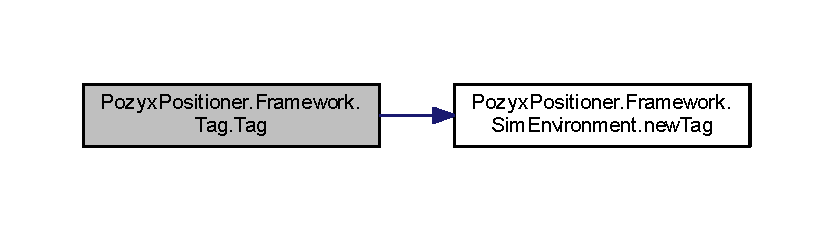
\includegraphics[width=350pt]{class_pozyx_positioner_1_1_framework_1_1_tag_a9b58a1a5756bf3c8cda1e2afd32276b2_cgraph}
\end{center}
\end{figure}


\subsection{Member Function Documentation}
\mbox{\Hypertarget{class_pozyx_positioner_1_1_framework_1_1_tag_ac2741e137c420ad71f64ee2d3d5fefe8}\label{class_pozyx_positioner_1_1_framework_1_1_tag_ac2741e137c420ad71f64ee2d3d5fefe8}} 
\index{Pozyx\+Positioner\+::\+Framework\+::\+Tag@{Pozyx\+Positioner\+::\+Framework\+::\+Tag}!Add\+Data@{Add\+Data}}
\index{Add\+Data@{Add\+Data}!Pozyx\+Positioner\+::\+Framework\+::\+Tag@{Pozyx\+Positioner\+::\+Framework\+::\+Tag}}
\subsubsection{\texorpdfstring{Add\+Data()}{AddData()}}
{\footnotesize\ttfamily void Pozyx\+Positioner.\+Framework.\+Tag.\+Add\+Data (\begin{DoxyParamCaption}\item[{\hyperlink{struct_pozyx_positioner_1_1_framework_1_1_pos_data}{Pos\+Data}}]{data }\end{DoxyParamCaption})}



Adds data to this tag\textquotesingle{}s positional data list, normalizes the data. Then calculates the best possible realtime position 


\begin{DoxyParams}{Parameters}
{\em data} & the \hyperlink{struct_pozyx_positioner_1_1_framework_1_1_pos_data}{Pos\+Data} to add to the list\\
\hline
\end{DoxyParams}
Here is the caller graph for this function\+:\nopagebreak
\begin{figure}[H]
\begin{center}
\leavevmode
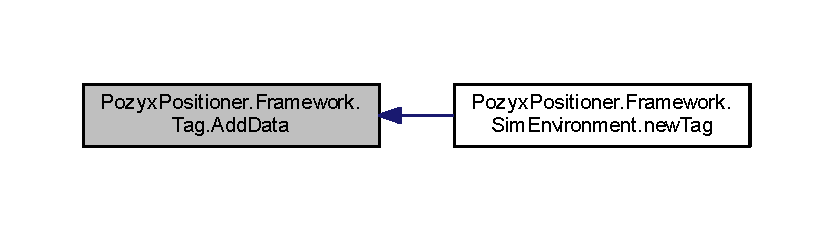
\includegraphics[width=350pt]{class_pozyx_positioner_1_1_framework_1_1_tag_ac2741e137c420ad71f64ee2d3d5fefe8_icgraph}
\end{center}
\end{figure}


\subsection{Property Documentation}
\mbox{\Hypertarget{class_pozyx_positioner_1_1_framework_1_1_tag_a0d75eeca4dea7088e2b4a60230c13012}\label{class_pozyx_positioner_1_1_framework_1_1_tag_a0d75eeca4dea7088e2b4a60230c13012}} 
\index{Pozyx\+Positioner\+::\+Framework\+::\+Tag@{Pozyx\+Positioner\+::\+Framework\+::\+Tag}!ID@{ID}}
\index{ID@{ID}!Pozyx\+Positioner\+::\+Framework\+::\+Tag@{Pozyx\+Positioner\+::\+Framework\+::\+Tag}}
\subsubsection{\texorpdfstring{ID}{ID}}
{\footnotesize\ttfamily string Pozyx\+Positioner.\+Framework.\+Tag.\+ID\hspace{0.3cm}{\ttfamily [get]}}



the ID of the tag 

\mbox{\Hypertarget{class_pozyx_positioner_1_1_framework_1_1_tag_a0b1b836b4e64ae70171587a2bcde4d71}\label{class_pozyx_positioner_1_1_framework_1_1_tag_a0b1b836b4e64ae70171587a2bcde4d71}} 
\index{Pozyx\+Positioner\+::\+Framework\+::\+Tag@{Pozyx\+Positioner\+::\+Framework\+::\+Tag}!Position@{Position}}
\index{Position@{Position}!Pozyx\+Positioner\+::\+Framework\+::\+Tag@{Pozyx\+Positioner\+::\+Framework\+::\+Tag}}
\subsubsection{\texorpdfstring{Position}{Position}}
{\footnotesize\ttfamily \hyperlink{struct_pozyx_positioner_1_1_framework_1_1_pozyx_vector}{Pozyx\+Vector} Pozyx\+Positioner.\+Framework.\+Tag.\+Position\hspace{0.3cm}{\ttfamily [get]}}



the current position of the tag 

\mbox{\Hypertarget{class_pozyx_positioner_1_1_framework_1_1_tag_a9010e57016df0a932c5ce8f8584ff5f9}\label{class_pozyx_positioner_1_1_framework_1_1_tag_a9010e57016df0a932c5ce8f8584ff5f9}} 
\index{Pozyx\+Positioner\+::\+Framework\+::\+Tag@{Pozyx\+Positioner\+::\+Framework\+::\+Tag}!refresh\+Rate@{refresh\+Rate}}
\index{refresh\+Rate@{refresh\+Rate}!Pozyx\+Positioner\+::\+Framework\+::\+Tag@{Pozyx\+Positioner\+::\+Framework\+::\+Tag}}
\subsubsection{\texorpdfstring{refresh\+Rate}{refreshRate}}
{\footnotesize\ttfamily int Pozyx\+Positioner.\+Framework.\+Tag.\+refresh\+Rate\hspace{0.3cm}{\ttfamily [get]}, {\ttfamily [set]}}



The refresh rate of the tag 



The documentation for this class was generated from the following file\+:\begin{DoxyCompactItemize}
\item 
Project/\+Pozyx\+Positioner/\+Pozyx\+Positioner/Sim\+Object.\+cs\end{DoxyCompactItemize}

%--- End generated contents ---

% Index
\backmatter
\newpage
\phantomsection
\clearemptydoublepage
\addcontentsline{toc}{chapter}{Index}
\printindex

\end{document}
